\chapter{Introdução}
\label{chp:introduction}

\begin{quotation}[]{Charlie Chaplin}
Don't be afraid of the unknown because even when they wander into chaos, planets are born stars.
\end{quotation}

Com o desenvolvimento crescente de aplicações para a Web Social, é notável o crescimento exponencial de dados heterogêneos na Web.
Com a grande produção de conteúdo nas redes sociais e o crescimento do acesso através de dispositivos móveis, surge uma variedade de informações que não são capazes de consumir completamente. Para ilustrar esse quadro, em um minuto \footnote{http://www.smartinsights.com/internet-marketing-statistics/happens-online-60-seconds/} o \textit{Facebook} tem 3.3 milhões de novos posts, são enviadas 29 milhões de mensagens no \textit{WhatsApp} e a plataforma de vídeos \textit{YouTube} tem uploads de quase 500 horas.
Há uma hora atrás \footnote{http://www.smartinsights.com/internet-marketing-statistics/real-time-mobile-usage-statistics-infographic/}, 3 milhões de fotos foram carregadas no \textit{Instagram} e houve 17 milhões de novos \textit{tweets} de dispositivos móveis no Twitter. A cada ano, são feitas mais de 148 milhões de reservas de viagens via Internet \footnote{http://www.statisticbrain.com/internet-travel-hotel-booking-statistics/} e o \textit{Google Maps} tem um total de visitas \footnote{https://www.similarweb.com/website/maps.google.com} de quase 79 milhões de usuários.

Com tantas informações disponíveis nem sempre é possível distinguir o que é de interesse de um e o que não é, um fenômeno da sobrecarga de informações. Na área de turismo, as pessoas tem interesses diversos e esses podem variar de acordo com o perfil de cada um ou de cada grupo. Uma pessoa seguindo um roteiro turístico padrão nem sempre estará satisfeita totalmente, pois o mesmo não é personalizado. Diante desse caso, Sistemas de Recomendação são ferramentas que podem auxiliar na filtragem de informações, respeitando o interesse de cada indivíduo.

De acordo com \cite{DiNoia2015}, Sistemas de Recomendações são uma família de ferramentas de filtragem de informações que auxiliam a encontrar, de forma personalizada, o que é relevante em um grande espaço de informações complexos. Ou seja, um sistema de recomendação fornece sugestões para escolher filmes, livros, músicas e, no contexto desse trabalho, rotas de pontos turísticos. Os Sistemas de Recomendação estão presentes no dia-a-dia em diversos serviços, seja no \textit{e-Commerce}, na apresentação de produtos que se assemelham ao que é  adquirido em determinado site; seja em \textit{e-Resource}, com a proposta de filmes, séries, músicas, livros e jogos.

A utilização de Sistemas de Recomendação se aplicam para diversas áreas além das que são conhecidas e experimentadas diariamente. Ela é aplicável em \textit{e-Library}, ajudando os usuários a selecionar fontes de conhecimento; \textit{e-Learning}, auxiliando alunos e professores a escolher assuntos e enriquecendo as atividades de aprendizado; e \textit{e-Tourism}, que são projetados para fornecer sugestões para turistas, como mobilidade, restaurantes, hospedagem, além de pontos de interesses a turistas geralmente baseado em popularidade, o que nem sempre é personalizado \citep{Singh2015}.

Além disso, é possível utilizar as informações fornecidas por outros serviços para indicar pontos turísticos a serem visitados. Por exemplo, existe a possibilidade de usar as avaliações que os usuários deram a um ponto turístico para indicar este local a um novo usuário.
\textit{Foursquare} \footnote{https://foursquare.com} é uma rede social que permite ao usuário avaliar e opinar sobre restaurantes, museus, praias e outros locais, além de ser um guia de cidades. Outros exemplos parecidos são o \textit{TripAdvisor} \footnote{https://www.tripadvisor.com} e Kekanto \footnote{https://kekanto.com.br}.

Uma característica de sistemas de recomendação, principalmente aqueles voltados para \textit{smartphones}, é que eles utilizam a localização geográfica para traçar rotas entre a origem e o destino. Entretanto, essas aplicações são limitadas e carecem de inteligência para prover uma melhor experiência para o usuário, assim pontos interessantes de visitação são "esquecidos" pelas rotas sugeridas.

Com o aumento do uso de dispositivos móveis, o sistema de \textit{e-Tourism} se tornou uma ótima oportunidade para serviços mobiles que auxiliam os turistas através de recomendações baseadas em suas preferências, sua localização e o contexto que está inserido. Um exemplo é o \textit{Google Trip} \footnote{https://get.google.com/trips/}, no qual o aplicativo planeja a viagem, desde hospedagem e passagem até a indicação de lugares na cidade, tanto para visitas como na organização da sua viagem, com recomendações de rotas.
\newline

\section{Problema}
\label{sec:problemIntroduction}

Este trabalho visa otimizar o uso de localização geográfica para recomendação de pontos turísticos em aplicações de apoio ao turismo.
Existem diversos serviços que auxiliam os usuários a planejarem suas viagens, porém muitos deles não oferecem ferramentas de filtragem ou as diversas opções de locais e serviços que o turista pode visitar durante a viagem.

A grande maioria desses sistemas constroem rotas para conhecer pontos turísticos com base na importância de cada um deles, seja no quesito histórico, valor cultural, beleza natural ou para entretenimento e diversão. A falta de informação de pontos turísticos leva pessoas a percorrerem longas distâncias ao invés de seguir por um caminho que contém pontos que seguem suas preferências e que pode ser feito em um tempo menor comparado as rotas padrões.

Um outro problema é que os pontos turísticos não mostram a vantagem de um deslocamento espacial em função do tempo, apenas listam os lugares sem apresentar melhores rotas baseado na localização da pessoa. Com tantas possibilidades a disposição, existe a dificuldade de montar um percurso que atenda as necessidades do viajante. De acordo com a sua localização espacial, o usuário deve ser capaz de selecionar a avaliação de outros usuários, a facilidade de mobilidade para determinadas atrações, horário de funcionamento, preços e entre outras informações.

\section{Objetivos da Solução Proposta}
\label{objectiveIntroduction}

O objetivo deste trabalho é o desenvolver um sistema de recomendação de rotas de pontos turísticos baseado em um algoritmo de filtragem colaborativa. Com isso espera-se melhorar as sugestões de passeios de turistas em união com as escolhas do viajante. Para gerar o perfil do usuário, serão utilizados seus dados das redes sociais de geolocalização ou redes geossociais, que pode conter o problema \textit{cold-start}, quando o sistema precisa de avaliações anteriores para oferecer bons resultados ao viajante.

O sistema realizará recomendações ao usuário coletando informações do perfil do usuário em relação às suas preferências de locais; possíveis avaliações feitas nas redes geossociais; e sua atual localização. Inicialmente, os conhecimentos absorvidos no perfil não serão suficientes para relacionar com os outros itens, mas utilizando serviços de APIs para obter informações estruturadas, será possível fazer a classificação.

Para exemplificar, suponha um turista que se encontra na Sorveteria da Ribeira e tem como destino o Museu de Arte Moderna da Bahia. Seguindo a rota padrão da Figura \ref{fig:route_default}, outro ponto turístico que poderá conhecer e que seja da sua preferência será o Mercado Modelo. Mas, caso o turista goste de visitar igrejas, é possível desviar o caminho para visitar a Igreja do Senhor do Bonfim e a Igreja de Nossa Senhora do Monte Serrat, pontos próximos do ponto de origem.

Os objetivos específicos para este trabalho são: 1) extração de dados de pontos de interesse e de usuários que avaliaram esses pontos; 2) o desenvolvimento de um sistema de recomendação de pontos turísticos de acordo com as preferências do usuário; e 3) gerar rota com base nos resultados do sistema de recomendação.

\begin{figure}[h!]
	\centering
	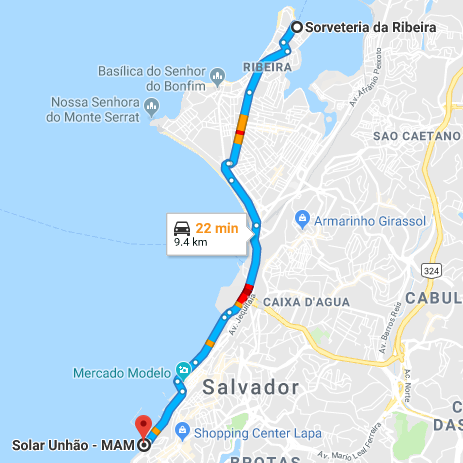
\includegraphics[scale=0.63]{images/image_2018-04-06_01-20-19.png}
	\caption{Rota gerada no Google Maps.}
	\label{fig:route_default}
\end{figure}

\section{Sumário}
\label{sec:summaryIntroduction}

Neste capítulo motiva-se e introduz o problema que este trabalho propõe resolver. Os próximos capítulos estão organizados da seguinte maneira: o capítulo \ref{chp:recSys} apresenta os conceitos teóricos usados neste trabalho referentes a Sistemas de Recomendação. O capítulo \ref{chp:eTourism} apresenta conceitos sobre Sistemas de Recomendação aplicados em Geolocalização. O capítulo \ref{chp:eTourismRecSys} apresenta a proposta de aplicação de sistemas de recomendação baseado em filtragem colaborativa em sugestões de rotas de pontos turísticos, além de discutir como foi feita a implementação. O capítulo \ref{chp:evaluation} apresenta a avaliação da ferramenta, conclusões e considerações finais.